\section{Direct Detection }
\label{sec:direct}
\ADW{Some introduction and context is needed here. Much of Lina's intro could be moved here.}

\subsection{Baryon Scattering \Contact{Vera}}
\Contributors{Vera, Kim, Lina N.}

The most sensitive low-energy searches for dark matter are looking to directly detect collisions of dark matter particles from the local galactic halo in underground detectors \citep{2013arXiv1310.8327C}. 
They have unprecedented sensitivity to WIMPs with masses well above a GeV, but the current generation of experiments is largely insensitive to lighter particles, for kinematic reasons. 
New technologies are necessary to open up sub-GeV models of dark matter to detailed exploration \citep{Battaglieri:2017aum}. 
Moreover, due to the extensive shielding of their targets, direct detection experiments have a ceiling on their sensitivity to large cross sections. 
The portion of dark matter parameter space excluded by current null results is shown in \figref{dd}. 
\begin{figure}
\centering
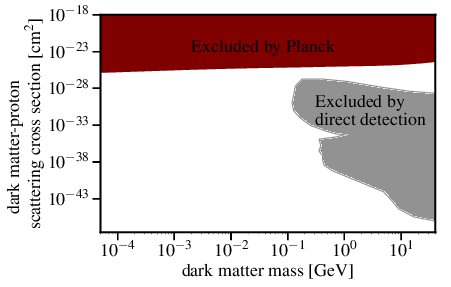
\includegraphics[width=0.6\columnwidth]{figures/planck_dd.png}
\caption{Currently-excluded regions of dark matter parameter space (mass versus cross section for scattering with protons through a velocity-independent spin-independent contact interaction) are shown as shaded regions. Gray region is excluded by various direct detection null results \citep{2018PhRvD..97l3013K} and red is excluded by CMB measurements \citep{Gluscevic:2017ywp}. We note that there are other limits in the same parameter space, but we choose to compare only these two, for illustration of complementarity between cosmological and low-energy laboratory searches.}
\label{fig:dd}
\end{figure}

Current null results from targeted laboratory searches motivate broad scans of parameter space that is inaccessible to underground experiments. Cosmological and astrophysical observables provide such a complementary search strategy. In particular, they are sensitive to scattering of sub-GeV particles with baryons at any point in cosmic history. Furthermore, there is no upper boundary on the interaction cross section they can probe. Finally, they are not subject to the uncertainty on local astrophysical properties of dark matter particles (their phase-space distribution), which affects the inferred limits on the particle properties of dark matter. 

If dark matter particles scatter with baryons, they transfer momentum between the two cosmological fluids, affecting density fluctuations and suppressing power at small scales; the power suppression can be captured by a variety of observables. The current limits come from the CMB \citep{Gluscevic:2017ywp}, cosmic-ray \citep{Cappiello:2018hsu}, and Lyman-$\alpha$ forest measurements \citep{Xu:2018efh}. For illustration, Figure \ref{fig:dd} compares currently excluded regions of dark matter parameter space, from analyses of Planck data, and from null results of various direct-detection searches.\footnote{We caution the reader that this is not a comprehensive list of current upper limits, but only serves to illustrate complementarity of cosmological and direct detection probes.} LSST will deliver state-of-the-art measurements of observables that trace matter fluctuations on a range of smaller scales, extending the sensitivity of astrophysical and cosmological searches far beyond the reach of Planck.

\subsection{Local Dark Matter Velocity Distribution \Contact{Lina}}
\Contributors{Lina N.}

%One way to detect dark matter (DM) is a process called direct detection, where DM particles scatter off heavy nuclei, emitting scintillation/ionization light that provide a direct signal of DM \citep{Goodman:1984dc}. 

The signal strength of dark matter (DM) scattering in direct detection experiments depends on both the local DM density and the DM velocity distribution. In this section we focus on the DM velocity distribution.

The differential rate with respect to the recoil energy $dR/dQ$ depends on the integral of the DM velocity distribution, $f(v)$, as
\begin{equation}
    \frac{dR}{dQ} \propto \int_{v_{\rm{min}}}^{v_{\rm{esc}}} \frac{f(v)}{v} dv, 
\end{equation}
where $v_{\rm{min}} = \sqrt{Q m_N/ (2 \mu^2)}$, with $Q$ the recoil energy, $m_N$ the mass of the nucleus against which DM is scattering, and $\mu = (m_N m_\chi / (m_N + m_\chi))$ the reduced mass of the nucleus $m_N$ and the DM mass $m_\chi$.

A novel method has recently been proposed to use the stars as tracers for the DM velocity \citep{Herzog-Arbeitman:2017fte,Necib:2018b}. These papers suggest that since accreted DM and stars have a comment origin, and are both collisionless, accreted stars are able to trace the velocity distribution of DM. This correlation holds for both the relaxed component of the DM, traced by older metal poor stars, and DM velocity substructure called debris flow traced by less metal poor stars from more recent mergers \citep{Lisanti:2011as,Kuhlen:2012fz,Lisanti:2014dva}. 

This method has already been applied on RAVE-TGAS data \citep{Herzog-Arbeitman:2017zbm}, and the second data release of Gaia in \cite{necib2018}. It has been found that the relaxed component of the DM although isotropic, has a mean speed lower than that of the assumed Maxwell Boltzmann distribution, reducing current limits by direct detection experiments \citep{Aprile:2018dbl}.

Another interesting aspect is the ability to reconstruct of more recent mergers. Using the second data release of Gaia, a new merger called the Gaia Sausage or the Gaia Enceleadus \citep{2018MNRAS.477.1472B,2018Natur.563...85H} has been found. Using the correlation observed in simulations, \cite{necib2018} extracted the new velocity distribution of DM brought in by the same merger, and studied its implications in current direct detection experiments. 

In order to do obtain the full empirical distribution of DM, one needs the 3-d velocities of the stars in the local neighborhood. Gaia provides proper motion and parallaxes for stars down to 20th magnitude. LSST will be able to extend this dataset to fainter stars, giving us a more accurate measurement of proper motions of stars in the solar neighborhood and beyond.

 Using proper motions of stars from LSST, coupled with radial velocity measurements from future telescopes like MSE, we will be able to obtain the most accurate 3-d velocity measurements of the local stars, and subsequently use this information to obtain a full empirical measurement of DM. Such detailed analysis will unveil new structures much smaller than the Gaia Sausage, but with equal importance in DM direct detection if it passes by the Solar neighborhood.
